% Generated by Sphinx.
\def\sphinxdocclass{report}
\documentclass[letterpaper,10pt,english]{sphinxmanual}
\usepackage[utf8]{inputenc}
\DeclareUnicodeCharacter{00A0}{\nobreakspace}
\usepackage[T1]{fontenc}
\usepackage{babel}
\usepackage{times}
\usepackage[Bjarne]{fncychap}
\usepackage{longtable}
\usepackage{sphinx}
\usepackage{multirow}


\title{CABS Documentation}
\date{July 06, 2012}
\release{2012}
\author{Andrzej Koliński}
\newcommand{\sphinxlogo}{}
\renewcommand{\releasename}{Release}
\makeindex

\makeatletter
\def\PYG@reset{\let\PYG@it=\relax \let\PYG@bf=\relax%
    \let\PYG@ul=\relax \let\PYG@tc=\relax%
    \let\PYG@bc=\relax \let\PYG@ff=\relax}
\def\PYG@tok#1{\csname PYG@tok@#1\endcsname}
\def\PYG@toks#1+{\ifx\relax#1\empty\else%
    \PYG@tok{#1}\expandafter\PYG@toks\fi}
\def\PYG@do#1{\PYG@bc{\PYG@tc{\PYG@ul{%
    \PYG@it{\PYG@bf{\PYG@ff{#1}}}}}}}
\def\PYG#1#2{\PYG@reset\PYG@toks#1+\relax+\PYG@do{#2}}

\expandafter\def\csname PYG@tok@gd\endcsname{\def\PYG@tc##1{\textcolor[rgb]{0.63,0.00,0.00}{##1}}}
\expandafter\def\csname PYG@tok@gu\endcsname{\let\PYG@bf=\textbf\def\PYG@tc##1{\textcolor[rgb]{0.50,0.00,0.50}{##1}}}
\expandafter\def\csname PYG@tok@gt\endcsname{\def\PYG@tc##1{\textcolor[rgb]{0.00,0.25,0.82}{##1}}}
\expandafter\def\csname PYG@tok@gs\endcsname{\let\PYG@bf=\textbf}
\expandafter\def\csname PYG@tok@gr\endcsname{\def\PYG@tc##1{\textcolor[rgb]{1.00,0.00,0.00}{##1}}}
\expandafter\def\csname PYG@tok@cm\endcsname{\let\PYG@it=\textit\def\PYG@tc##1{\textcolor[rgb]{0.25,0.50,0.56}{##1}}}
\expandafter\def\csname PYG@tok@vg\endcsname{\def\PYG@tc##1{\textcolor[rgb]{0.73,0.38,0.84}{##1}}}
\expandafter\def\csname PYG@tok@m\endcsname{\def\PYG@tc##1{\textcolor[rgb]{0.13,0.50,0.31}{##1}}}
\expandafter\def\csname PYG@tok@mh\endcsname{\def\PYG@tc##1{\textcolor[rgb]{0.13,0.50,0.31}{##1}}}
\expandafter\def\csname PYG@tok@cs\endcsname{\def\PYG@tc##1{\textcolor[rgb]{0.25,0.50,0.56}{##1}}\def\PYG@bc##1{\setlength{\fboxsep}{0pt}\colorbox[rgb]{1.00,0.94,0.94}{\strut ##1}}}
\expandafter\def\csname PYG@tok@ge\endcsname{\let\PYG@it=\textit}
\expandafter\def\csname PYG@tok@vc\endcsname{\def\PYG@tc##1{\textcolor[rgb]{0.73,0.38,0.84}{##1}}}
\expandafter\def\csname PYG@tok@il\endcsname{\def\PYG@tc##1{\textcolor[rgb]{0.13,0.50,0.31}{##1}}}
\expandafter\def\csname PYG@tok@go\endcsname{\def\PYG@tc##1{\textcolor[rgb]{0.19,0.19,0.19}{##1}}}
\expandafter\def\csname PYG@tok@cp\endcsname{\def\PYG@tc##1{\textcolor[rgb]{0.00,0.44,0.13}{##1}}}
\expandafter\def\csname PYG@tok@gi\endcsname{\def\PYG@tc##1{\textcolor[rgb]{0.00,0.63,0.00}{##1}}}
\expandafter\def\csname PYG@tok@gh\endcsname{\let\PYG@bf=\textbf\def\PYG@tc##1{\textcolor[rgb]{0.00,0.00,0.50}{##1}}}
\expandafter\def\csname PYG@tok@ni\endcsname{\let\PYG@bf=\textbf\def\PYG@tc##1{\textcolor[rgb]{0.84,0.33,0.22}{##1}}}
\expandafter\def\csname PYG@tok@nl\endcsname{\let\PYG@bf=\textbf\def\PYG@tc##1{\textcolor[rgb]{0.00,0.13,0.44}{##1}}}
\expandafter\def\csname PYG@tok@nn\endcsname{\let\PYG@bf=\textbf\def\PYG@tc##1{\textcolor[rgb]{0.05,0.52,0.71}{##1}}}
\expandafter\def\csname PYG@tok@no\endcsname{\def\PYG@tc##1{\textcolor[rgb]{0.38,0.68,0.84}{##1}}}
\expandafter\def\csname PYG@tok@na\endcsname{\def\PYG@tc##1{\textcolor[rgb]{0.25,0.44,0.63}{##1}}}
\expandafter\def\csname PYG@tok@nb\endcsname{\def\PYG@tc##1{\textcolor[rgb]{0.00,0.44,0.13}{##1}}}
\expandafter\def\csname PYG@tok@nc\endcsname{\let\PYG@bf=\textbf\def\PYG@tc##1{\textcolor[rgb]{0.05,0.52,0.71}{##1}}}
\expandafter\def\csname PYG@tok@nd\endcsname{\let\PYG@bf=\textbf\def\PYG@tc##1{\textcolor[rgb]{0.33,0.33,0.33}{##1}}}
\expandafter\def\csname PYG@tok@ne\endcsname{\def\PYG@tc##1{\textcolor[rgb]{0.00,0.44,0.13}{##1}}}
\expandafter\def\csname PYG@tok@nf\endcsname{\def\PYG@tc##1{\textcolor[rgb]{0.02,0.16,0.49}{##1}}}
\expandafter\def\csname PYG@tok@si\endcsname{\let\PYG@it=\textit\def\PYG@tc##1{\textcolor[rgb]{0.44,0.63,0.82}{##1}}}
\expandafter\def\csname PYG@tok@s2\endcsname{\def\PYG@tc##1{\textcolor[rgb]{0.25,0.44,0.63}{##1}}}
\expandafter\def\csname PYG@tok@vi\endcsname{\def\PYG@tc##1{\textcolor[rgb]{0.73,0.38,0.84}{##1}}}
\expandafter\def\csname PYG@tok@nt\endcsname{\let\PYG@bf=\textbf\def\PYG@tc##1{\textcolor[rgb]{0.02,0.16,0.45}{##1}}}
\expandafter\def\csname PYG@tok@nv\endcsname{\def\PYG@tc##1{\textcolor[rgb]{0.73,0.38,0.84}{##1}}}
\expandafter\def\csname PYG@tok@s1\endcsname{\def\PYG@tc##1{\textcolor[rgb]{0.25,0.44,0.63}{##1}}}
\expandafter\def\csname PYG@tok@gp\endcsname{\let\PYG@bf=\textbf\def\PYG@tc##1{\textcolor[rgb]{0.78,0.36,0.04}{##1}}}
\expandafter\def\csname PYG@tok@sh\endcsname{\def\PYG@tc##1{\textcolor[rgb]{0.25,0.44,0.63}{##1}}}
\expandafter\def\csname PYG@tok@ow\endcsname{\let\PYG@bf=\textbf\def\PYG@tc##1{\textcolor[rgb]{0.00,0.44,0.13}{##1}}}
\expandafter\def\csname PYG@tok@sx\endcsname{\def\PYG@tc##1{\textcolor[rgb]{0.78,0.36,0.04}{##1}}}
\expandafter\def\csname PYG@tok@bp\endcsname{\def\PYG@tc##1{\textcolor[rgb]{0.00,0.44,0.13}{##1}}}
\expandafter\def\csname PYG@tok@c1\endcsname{\let\PYG@it=\textit\def\PYG@tc##1{\textcolor[rgb]{0.25,0.50,0.56}{##1}}}
\expandafter\def\csname PYG@tok@kc\endcsname{\let\PYG@bf=\textbf\def\PYG@tc##1{\textcolor[rgb]{0.00,0.44,0.13}{##1}}}
\expandafter\def\csname PYG@tok@c\endcsname{\let\PYG@it=\textit\def\PYG@tc##1{\textcolor[rgb]{0.25,0.50,0.56}{##1}}}
\expandafter\def\csname PYG@tok@mf\endcsname{\def\PYG@tc##1{\textcolor[rgb]{0.13,0.50,0.31}{##1}}}
\expandafter\def\csname PYG@tok@err\endcsname{\def\PYG@bc##1{\setlength{\fboxsep}{0pt}\fcolorbox[rgb]{1.00,0.00,0.00}{1,1,1}{\strut ##1}}}
\expandafter\def\csname PYG@tok@kd\endcsname{\let\PYG@bf=\textbf\def\PYG@tc##1{\textcolor[rgb]{0.00,0.44,0.13}{##1}}}
\expandafter\def\csname PYG@tok@ss\endcsname{\def\PYG@tc##1{\textcolor[rgb]{0.32,0.47,0.09}{##1}}}
\expandafter\def\csname PYG@tok@sr\endcsname{\def\PYG@tc##1{\textcolor[rgb]{0.14,0.33,0.53}{##1}}}
\expandafter\def\csname PYG@tok@mo\endcsname{\def\PYG@tc##1{\textcolor[rgb]{0.13,0.50,0.31}{##1}}}
\expandafter\def\csname PYG@tok@mi\endcsname{\def\PYG@tc##1{\textcolor[rgb]{0.13,0.50,0.31}{##1}}}
\expandafter\def\csname PYG@tok@kn\endcsname{\let\PYG@bf=\textbf\def\PYG@tc##1{\textcolor[rgb]{0.00,0.44,0.13}{##1}}}
\expandafter\def\csname PYG@tok@o\endcsname{\def\PYG@tc##1{\textcolor[rgb]{0.40,0.40,0.40}{##1}}}
\expandafter\def\csname PYG@tok@kr\endcsname{\let\PYG@bf=\textbf\def\PYG@tc##1{\textcolor[rgb]{0.00,0.44,0.13}{##1}}}
\expandafter\def\csname PYG@tok@s\endcsname{\def\PYG@tc##1{\textcolor[rgb]{0.25,0.44,0.63}{##1}}}
\expandafter\def\csname PYG@tok@kp\endcsname{\def\PYG@tc##1{\textcolor[rgb]{0.00,0.44,0.13}{##1}}}
\expandafter\def\csname PYG@tok@w\endcsname{\def\PYG@tc##1{\textcolor[rgb]{0.73,0.73,0.73}{##1}}}
\expandafter\def\csname PYG@tok@kt\endcsname{\def\PYG@tc##1{\textcolor[rgb]{0.56,0.13,0.00}{##1}}}
\expandafter\def\csname PYG@tok@sc\endcsname{\def\PYG@tc##1{\textcolor[rgb]{0.25,0.44,0.63}{##1}}}
\expandafter\def\csname PYG@tok@sb\endcsname{\def\PYG@tc##1{\textcolor[rgb]{0.25,0.44,0.63}{##1}}}
\expandafter\def\csname PYG@tok@k\endcsname{\let\PYG@bf=\textbf\def\PYG@tc##1{\textcolor[rgb]{0.00,0.44,0.13}{##1}}}
\expandafter\def\csname PYG@tok@se\endcsname{\let\PYG@bf=\textbf\def\PYG@tc##1{\textcolor[rgb]{0.25,0.44,0.63}{##1}}}
\expandafter\def\csname PYG@tok@sd\endcsname{\let\PYG@it=\textit\def\PYG@tc##1{\textcolor[rgb]{0.25,0.44,0.63}{##1}}}

\def\PYGZbs{\char`\\}
\def\PYGZus{\char`\_}
\def\PYGZob{\char`\{}
\def\PYGZcb{\char`\}}
\def\PYGZca{\char`\^}
\def\PYGZam{\char`\&}
\def\PYGZlt{\char`\<}
\def\PYGZgt{\char`\>}
\def\PYGZsh{\char`\#}
\def\PYGZpc{\char`\%}
\def\PYGZdl{\char`\$}
\def\PYGZti{\char`\~}
% for compatibility with earlier versions
\def\PYGZat{@}
\def\PYGZlb{[}
\def\PYGZrb{]}
\makeatother

\begin{document}

\maketitle
\tableofcontents
\phantomsection\label{index::doc}

\index{pycabs (module)}\index{CABS (class in pycabs)}

\begin{fulllineitems}
\phantomsection\label{index:pycabs.CABS}\pysiglinewithargsret{\strong{class }\code{pycabs.}\bfcode{CABS}}{\emph{sequence}, \emph{secondary\_structure}, \emph{templates\_filenames}, \emph{project\_name}}{}
CABS main class.
\begin{quote}\begin{description}
\item[{Parameters}] \leavevmode\begin{itemize}
\item {} 
\textbf{sequence} (\emph{string}) -- one line sequence of the target protein

\item {} 
\textbf{secondary\_structure} (\emph{string}) -- one line secondary structure for the target protein

\item {} 
\textbf{templates\_filenames} (\emph{list}) -- path to 3D protein model templates in pdb file format which you want to use for modeling. C\(\alpha\) numbering in templates must be aligned to target sequence

\item {} 
\textbf{project\_name} (\emph{string}) -- project\_name and working directory name (uniq)

\end{itemize}

\end{description}\end{quote}
\index{calcConstraints() (pycabs.CABS method)}

\begin{fulllineitems}
\phantomsection\label{index:pycabs.CABS.calcConstraints}\pysiglinewithargsret{\bfcode{calcConstraints}}{\emph{exclude\_residues=}\optional{}, \emph{other\_constraints=}\optional{}}{}
Calculate distance constraints using templates 3D models.
\begin{quote}\begin{description}
\item[{Parameters}] \leavevmode\begin{itemize}
\item {} 
\textbf{exclude\_residues} (\emph{list}) -- indexes of residues without constrains

\item {} 
\textbf{constrains} (\emph{other}) -- user-defined constrains as list of tuples: (residue\_i\_index,residue\_j\_index,constraint\_strength)

\end{itemize}

\end{description}\end{quote}

\end{fulllineitems}

\index{convertPdbToDcd() (pycabs.CABS method)}

\begin{fulllineitems}
\phantomsection\label{index:pycabs.CABS.convertPdbToDcd}\pysiglinewithargsret{\bfcode{convertPdbToDcd}}{\emph{catdcd\_path='/home/hydek/pycabs/FF/catdcd'}}{}
This is only simple wrapper to CatDCD software (\href{http://www.ks.uiuc.edu/Development/MDTools/catdcd/}{http://www.ks.uiuc.edu/Development/MDTools/catdcd/}), 
could be usable since *.dcd binary format is few times lighter than pdb, and many python libraries 
(ProDy, MDAnalysis) use *.dcd as trajectory input format.
Before use, download CatDCD from \href{http://www.ks.uiuc.edu/Development/MDTools/catdcd/}{http://www.ks.uiuc.edu/Development/MDTools/catdcd/} and modify catdcd\_path.

\end{fulllineitems}

\index{createLatticeReplicas() (pycabs.CABS method)}

\begin{fulllineitems}
\phantomsection\label{index:pycabs.CABS.createLatticeReplicas}\pysiglinewithargsret{\bfcode{createLatticeReplicas}}{\emph{start\_structures\_fn=}\optional{}, \emph{replicas=20}}{}
Create protein models projected onto CABS lattice, which will be used as replicas.
\begin{quote}\begin{description}
\item[{Parameters}] \leavevmode\begin{itemize}
\item {} 
\textbf{start\_structures\_fn} (\emph{list}) -- list of paths to pdb files which should be used instead of templates models.  This parameter is optional, and probably not often used. Without it script creates replicas from templates files.

\item {} 
\textbf{replicas} (\emph{integer}) -- define number of replicas in CABS simulation. However 20 is optimal for most cases, and you don't need to change it in protein modeling case.

\end{itemize}

\end{description}\end{quote}

\begin{notice}{note}{Note:}
If number of replicas is smaller than number of templates - program will create replicas using first \emph{replicas} templates. If there is less templates than replicas, they are creating sequentially using template models.
\end{notice}

\end{fulllineitems}

\index{rng\_seed (pycabs.CABS attribute)}

\begin{fulllineitems}
\phantomsection\label{index:pycabs.CABS.rng_seed}\pysigline{\bfcode{rng\_seed}\strong{ = None}}
seed for random generator

\end{fulllineitems}

\index{trafToPdb() (pycabs.CABS method)}

\begin{fulllineitems}
\phantomsection\label{index:pycabs.CABS.trafToPdb}\pysiglinewithargsret{\bfcode{trafToPdb}}{\emph{output\_filename='TRAF.pdb'}}{}
Convert TRAF CABS pseudotrajectory file format into multimodel pdb

\end{fulllineitems}


\end{fulllineitems}

\index{Calculate (class in pycabs)}

\begin{fulllineitems}
\phantomsection\label{index:pycabs.Calculate}\pysiglinewithargsret{\strong{class }\code{pycabs.}\bfcode{Calculate}}{\emph{output}}{}
Inherit if you want to process data used with {\hyperref[index:pycabs.Monitor]{\code{Monitor}}} class.
\begin{quote}\begin{description}
\item[{Parameters}] \leavevmode
\textbf{output} (\emph{array/list}) -- output array with calculated results

\end{description}\end{quote}
\index{processTrajectory() (pycabs.Calculate method)}

\begin{fulllineitems}
\phantomsection\label{index:pycabs.Calculate.processTrajectory}\pysiglinewithargsret{\bfcode{processTrajectory}}{\emph{data}}{}
Use it in \emph{calculate} method if you parsing TRAF file, and want to calculate something on structure
\begin{quote}\begin{description}
\item[{Result }] \leavevmode
Array of 1D model coordinates

\end{description}\end{quote}

\end{fulllineitems}


\end{fulllineitems}

\index{Errors}

\begin{fulllineitems}
\phantomsection\label{index:pycabs.Errors}\pysiglinewithargsret{\strong{exception }\code{pycabs.}\bfcode{Errors}}{\emph{value}}{}
Simple error messages

\end{fulllineitems}

\index{Info (class in pycabs)}

\begin{fulllineitems}
\phantomsection\label{index:pycabs.Info}\pysiglinewithargsret{\strong{class }\code{pycabs.}\bfcode{Info}}{\emph{text}}{}
Simple message system

\end{fulllineitems}

\index{Monitor (class in pycabs)}

\begin{fulllineitems}
\phantomsection\label{index:pycabs.Monitor}\pysiglinewithargsret{\strong{class }\code{pycabs.}\bfcode{Monitor}}{\emph{filename}, \emph{calculate}}{}
Class for monitoring of CABS output data. You can run it and dynamically update output arrays with calculated results.
\begin{quote}\begin{description}
\item[{Parameters}] \leavevmode
\textbf{calculate} ({\hyperref[index:pycabs.Calculate]{\code{Calculate}}}) -- what to do with gathered data ?

\end{description}\end{quote}
\index{daemon (pycabs.Monitor attribute)}

\begin{fulllineitems}
\phantomsection\label{index:pycabs.Monitor.daemon}\pysigline{\bfcode{daemon}\strong{ = None}}
if True, it will terminate when script terminates

\end{fulllineitems}

\index{run() (pycabs.Monitor method)}

\begin{fulllineitems}
\phantomsection\label{index:pycabs.Monitor.run}\pysiglinewithargsret{\bfcode{run}}{}{}
Run monitor in background

\end{fulllineitems}

\index{terminate() (pycabs.Monitor method)}

\begin{fulllineitems}
\phantomsection\label{index:pycabs.Monitor.terminate}\pysiglinewithargsret{\bfcode{terminate}}{}{}
Terminate monitor

\end{fulllineitems}


\end{fulllineitems}

\index{parsePorterOutput() (in module pycabs)}

\begin{fulllineitems}
\phantomsection\label{index:pycabs.parsePorterOutput}\pysiglinewithargsret{\code{pycabs.}\bfcode{parsePorterOutput}}{\emph{porter\_output\_fn}}{}
Porter (protein secondary stucture prediction, \href{http://distill.ucd.ie/porter/}{http://distill.ucd.ie/porter/}) output parser. 
Porter emailed output looks like:

\begin{Verbatim}[commandchars=\\\{\}]
\PYG{n}{IDVLLGADDGSLAFVPSEFSISPGEKIVFKNNAGFPHNIVFDEDSIPSGVDASKISMSEE}
\PYG{n}{CEEEECCCCCCCCEECCEEEECCCCEEEEEECCCCCEEEEECCCCCCCCCCHHHHCCCCC}



\PYG{n}{DLLNAKGETFEVALSNKGEYSFYCSPHQGAGMVGKVTVN}
\PYG{n}{CCECCCCCEEEEECCCCEEEEEECCHHHHCCCEEEEEEC}
\end{Verbatim}
\begin{quote}\begin{description}
\item[{Parameters}] \leavevmode
\textbf{porter\_output\_fn} (\emph{string}) -- path to the porter output file

\item[{Returns}] \leavevmode
tuple (sequence, secondary\_structure)

\end{description}\end{quote}

\end{fulllineitems}

\index{parsePsipredOutput() (in module pycabs)}

\begin{fulllineitems}
\phantomsection\label{index:pycabs.parsePsipredOutput}\pysiglinewithargsret{\code{pycabs.}\bfcode{parsePsipredOutput}}{\emph{psipred\_output\_fn}}{}
Psipred (protein secondary structure prediction, \href{http://bioinf.cs.ucl.ac.uk/psipred/}{http://bioinf.cs.ucl.ac.uk/psipred/}) output parser. 
Psipred output looks like:

\begin{Verbatim}[commandchars=\\\{\}]
\textgreater{} head psipred.ss
1 P C   1.000  0.000  0.000
2 K C   0.665  0.000  0.459
3 A E   0.018  0.000  0.991
4 L E   0.008  0.000  0.997
5 I E   0.002  0.000  0.998
6 V E   0.003  0.000  0.999
7 Y E   0.033  0.000  0.981
\end{Verbatim}
\begin{quote}\begin{description}
\item[{Parameters}] \leavevmode
\textbf{psipred\_output\_fn} (\emph{string}) -- path to the psipred output file

\item[{Returns}] \leavevmode
tuple (sequence, secondary\_structure)

\end{description}\end{quote}

\end{fulllineitems}


Contents:

\begin{Verbatim}[commandchars=\\\{\}]
\PYG{k+kn}{from} \PYG{n+nn}{pylab} \PYG{k+kn}{import} \PYG{o}{*}
\PYG{k+kn}{from} \PYG{n+nn}{matplotlib.patches} \PYG{k+kn}{import} \PYG{n}{Ellipse}

\PYG{n}{delta} \PYG{o}{=} \PYG{l+m+mf}{45.0} \PYG{c}{\PYGZsh{} degrees}

\PYG{n}{angles} \PYG{o}{=} \PYG{n}{arange}\PYG{p}{(}\PYG{l+m+mi}{0}\PYG{p}{,} \PYG{l+m+mi}{360}\PYG{o}{+}\PYG{n}{delta}\PYG{p}{,} \PYG{n}{delta}\PYG{p}{)}
\PYG{n}{ells} \PYG{o}{=} \PYG{p}{[}\PYG{n}{Ellipse}\PYG{p}{(}\PYG{p}{(}\PYG{l+m+mi}{1}\PYG{p}{,} \PYG{l+m+mi}{1}\PYG{p}{)}\PYG{p}{,} \PYG{l+m+mi}{4}\PYG{p}{,} \PYG{l+m+mi}{2}\PYG{p}{,} \PYG{n}{a}\PYG{p}{)} \PYG{k}{for} \PYG{n}{a} \PYG{o+ow}{in} \PYG{n}{angles}\PYG{p}{]}

\PYG{n}{a} \PYG{o}{=} \PYG{n}{subplot}\PYG{p}{(}\PYG{l+m+mi}{111}\PYG{p}{,} \PYG{n}{aspect}\PYG{o}{=}\PYG{l+s}{'}\PYG{l+s}{equal}\PYG{l+s}{'}\PYG{p}{)}

\PYG{k}{for} \PYG{n}{e} \PYG{o+ow}{in} \PYG{n}{ells}\PYG{p}{:}
    \PYG{n}{e}\PYG{o}{.}\PYG{n}{set\PYGZus{}clip\PYGZus{}box}\PYG{p}{(}\PYG{n}{a}\PYG{o}{.}\PYG{n}{bbox}\PYG{p}{)}
    \PYG{n}{e}\PYG{o}{.}\PYG{n}{set\PYGZus{}alpha}\PYG{p}{(}\PYG{l+m+mf}{0.1}\PYG{p}{)}
    \PYG{n}{a}\PYG{o}{.}\PYG{n}{add\PYGZus{}artist}\PYG{p}{(}\PYG{n}{e}\PYG{p}{)}

\PYG{n}{xlim}\PYG{p}{(}\PYG{o}{-}\PYG{l+m+mi}{2}\PYG{p}{,} \PYG{l+m+mi}{4}\PYG{p}{)}
\PYG{n}{ylim}\PYG{p}{(}\PYG{o}{-}\PYG{l+m+mi}{1}\PYG{p}{,} \PYG{l+m+mi}{3}\PYG{p}{)}

\PYG{n}{show}\PYG{p}{(}\PYG{p}{)}
\end{Verbatim}
\begin{figure}[htbp]
\centering

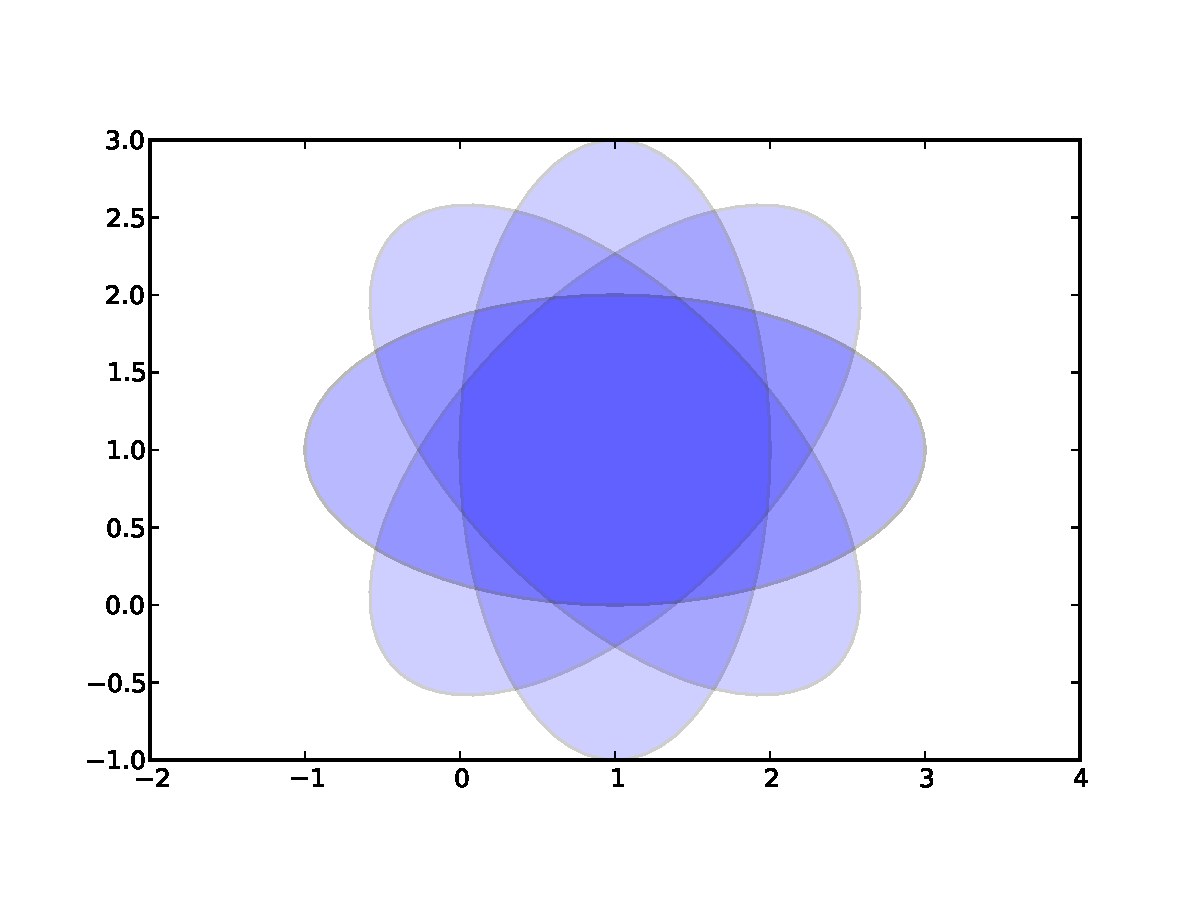
\includegraphics{ellipses.pdf}
\end{figure}


\chapter{Indices and tables}
\label{index:welcome-to-cabs-s-documentation}\label{index::doc}\label{index:module-pycabs}\label{index:indices-and-tables}\begin{itemize}
\item {} 
\emph{genindex}

\item {} 
\emph{modindex}

\item {} 
\emph{search}

\end{itemize}


\renewcommand{\indexname}{Python Module Index}
\begin{theindex}
\def\bigletter#1{{\Large\sffamily#1}\nopagebreak\vspace{1mm}}
\bigletter{p}
\item {\texttt{pycabs}}, \pageref{index:module-pycabs}
\end{theindex}

\renewcommand{\indexname}{Index}
\printindex
\end{document}
